\section{Various}


\begin{tcolorbox}
	Standard Deviation = $\sqrt{\text{Variance}}$, Standard Deviation = $\sigma$, Variance = $\sigma^2$
\end{tcolorbox}


\subsection{Two-Sampled t-Test}

\subsubsection{Unpaired Data}

We have $X_i$ i.i.d. $\sim \mathcal N(\mu_X, \sigma^2)$ and $Y_j$ i.i.d. $\sim \mathcal N(\mu_Y, \sigma^2)$ with $X_i, Y_j$ independent. For the $t$-test, $H_0: \mu_X = \mu_Y$ and $H_A: \mu_X \neq \mu_Y$. Then:
$$T = \frac{\bar X_n - \bar Y_m}{\sqrt{\frac{s^2}{n} + \frac{s^2}{m}}} \sim t_{n+m-2} \text{ under } H_0$$

\subsubsection{Paired Data}

We have independent $D_i = X_i - Y_i$ and:
$$\bar D = \frac{1}{n} \sum_{i=1}^n D_i \sim \mathcal N(\mu_D, \sigma_D / \sqrt{n})$$

$H_0$ and $H_A$ as before and:
$$T = \sqrt{n} \frac{\bar D}{S_D} \sim t_{n-1} \text{ under } H_0$$

\subsection{Charts}

\begin{lstlisting}
stripchart(y ~ x, vertical = T, pch = 1, data = d)
boxplot(y ~ x, data = d)
with(d, interaction.plot(x.factor = a, trace.factor = b, response = y))
\end{lstlisting}

\textbf{If the lines of an interaction plot are NOT parallel, there is possibly an interaction effect we have to consider.}


\subsection{Data Generation / Calculations}
\begin{lstlisting}
## Generate 10 A's followed by 10 B's
rep(c("A", "B"), each = 10)

## Alternate A, B 10 times
rep(c("A", "B"), times = 10)

## Toss a coin 20 times (1/2 prob. for A, B)
sample(c("A", "B"), 20, replace = T)

## Choose 10 A's at random, the rest B's
sample(rep(c("A", "B"), times = 10), 20, replace = F)

## Overall mean of column A
mean(d$A) ## or aggreagte(A ~ 1, data = d, mean)

## Group mean per B
aggregate(A ~ B, data = d, mean)
\end{lstlisting}


\subsection{Examples}

\subsubsection{Split-Plot Design, ANOVA Skeleton}

Three new types of pizzas in six different packings are investigated by 90 consumers on a 0-10 scale. Each person rates the six packings of just one type of pizza, that is pizzas are randomized to persons and each person tastes the different packings in random order. \medskip

This is a split-plot design with persons as whole plots and rating orders (or time slots) as split plots. Pizza type is the whole-plot factor, packing the split-plot factor. We have:
$$Y_{ijk} = \mu + \beta_i + \eta_{k(i)} + \alpha_j + (\alpha \beta)_{ij} + \epsilon_{k(ij)}$$

Where $\eta_{k(i)}$ is the whole-plot error. The ANOVA skeleton is given by:
\begin{center}
	\includegraphics[width=\linewidth]{anova-skeleton.png}
\end{center}

\subsubsection{Split-Plot Design with Blocking}

A soil scientist wanted to investigate the effects of nitrogen supplied in four different forms and later evaluate those effects combined with those of thatch accumulation (two, five or eight years of accumulation) on the quality of an established turf. A golf green had been constructed and seeded with grass on the experimental plots. The nitrogen treatment plots were arranged on the golf green in a randomized complete block design with two block levels. Each of the eight experimental plots was split into three subplots to which the levels of the second treatment factor were randomly assigned. \medskip

This is a split-plot design with whole-plot factor nitrogen, split-plot factor thatch and a block factor block.
$$Y_{ijkl} = \mu + \gamma_i + \alpha_j + \beta_k + (\alpha \beta)_{jk} + \eta_{l(ij)} + \epsilon_{l(ijk)}$$

Where $l = 1$, $\gamma_i$ fixed effect of the block, $\alpha_j$ fixed main effect of nitrogen, $\beta_k$ fixed main effect of thatch, $(\alpha \beta)_{jk}$ interaction, $\eta_{l(ij)}$ error on the whole-plot level and $\epsilon_{l(ijk)}$ the error on the split-plot level. \medskip


\hrulefill

\textbf{Ex.} We fitted the RCB experiment and plot \texttt{plot(TukeyHSD(x = "fit", "treatment", conf.level = 0.95))}. \medskip

\begin{wrapfigure}[10]{l}{0.4\linewidth}
    \vspace{-15pt}
    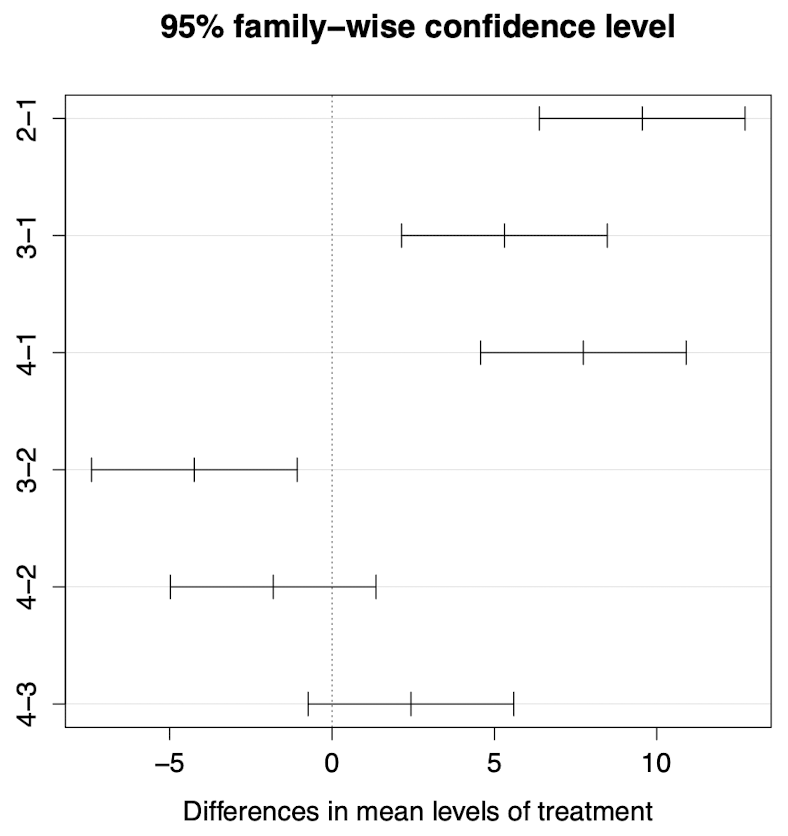
\includegraphics[width=1.15\linewidth]{tukey_confint.png}
\end{wrapfigure}

Which treatment differences are significant?
\begin{itemize}
	\item[$\square$] $2-1, 3 - 1, 4 - 1$
	\item[$\square$] $3-2$
	\item[$\square$] $4-2, 4-3$
	\item[$\square$] $2-1$
	\item[$\boxtimes$] $2-1, 3-1, 4-1, 3-2$
\end{itemize}
Since a treatment difference is significant if the corresponding confidence interval does not cover 0.


\hrulefill

\textbf{Ex.} Given a two-way ANOVA model with a significant factor $A$, an insignificant factor $B$ and a significant interaction term. Can we remove any terms from the model? \medskip

No, we should not remove a significant term and since the interaction is significant we cannot remove the main effect $B$.


\hrulefill

\textbf{Ex.} When fitting two ANOVA models with \texttt{fit1 <- aov(y ~ age * educ, data = survey)} and \texttt{fit2 <- aov(y ~ educ * age, data = survey)}, we might encounter different $p$-values for both \texttt{age} and \texttt{educ}, what might be the reason? \medskip

If there is a difference, the design must be unbalanced. In that case, the type I sum of squares used in \texttt{aov()} is dependent on the order of how the variables appear in the model. The interaction has the same $p$-value because it is adjusted for \texttt{age} and \texttt{educ} in both cases.


\hrulefill

\textbf{Ex.} The mixed effect model $\text{Rating}_{ij} = \mu + \text{Type}_i + \text{Subject}_j + \epsilon_{ij}$ is used. Type is a fixed effect and Subject a random (block) factor. For fixed $j$, are the Rating$_{ij}$ uncorrelated? \medskip

No, they are not as subjects have an effect since $\text{Var}(\text{Subject}_i)) \neq 0$.


\hrulefill

\textbf{Ex.} Which statement about RCB is true:
\begin{itemize}
	\item[$\square$]  A RCB tries to ensure heterogeneity within blocks
	\item[$\boxtimes$] The error with $r$ blocks hard $r-1$ less DF than the error of a completely randomized design with the same number of experimental units.
	\item[$\square$] The number of experimental units in a block can be less than the number of treatments
	\item[$\square$] Can be constructed from a completely randomized design by imposing blocking after randomization
\end{itemize}


\hrulefill

\textbf{Ex.} Given three levels of a treatment, which design should be preferred if interested in difference of treatments (assuming the variance of the units is the same for both designs)?\smallskip

D1: 2 pieces of land with 3 sub-fields each and form 2 complete blocks\smallskip

D2: 3 pieces of land with 2 sub-fields each and form 3 blocks
\begin{itemize}
	\item[$\boxtimes$] D1 should be preferred
	\item[$\square$] D2 should be preferred
	\item[$\square$] There is no important difference between D1 and D2
\end{itemize}
The incomplete block design D2 has more variance in the estimates of treatment differences than the complete block design D1. Therefore D1 should be preferred.


\hrulefill

\textbf{Ex.} Consider a balanced one-way ANOVA model. What happens to the 95\%-quantile of the $F$-distribution of the global test if we increase the number of observations?
\begin{itemize}
	\item[$\square$] The quantile gets larger
	\item[$\boxtimes$] The quantile gets smaller
	\item[$\square$] The quantile stays the same
\end{itemize}


\hrulefill

\textbf{Ex.} Consider a test with 4 types of toothpaste and 3 types of packaging. 60 participants have been selected and each participant is supposed to test and rate every packaging of exactly one toothpaste type. Which type of design is this?
\begin{itemize}
	\item[$\boxtimes$] Split-plot design with participants as whole-plots
	\item[$\square$] Split-plot design with toothpaste as whole-plots
	\item[$\square$] Split-plot design with packagings as whole-plots
\end{itemize}


\hrulefill

\textbf{Ex.} Consider the following experimental design with a treatment factor having levels $A, B, C, D, E, F$. Which of the statements is true?
\begin{center}
	\begin{tabular}{c | c  | c | c | c | c}
		 Block 1 & Block 2 & Block 3 & Block 4 & Block 5 & Block 6\\ \hline
		 A & A & B & D & D & B \\
		 B & C & C & E & F & F
	\end{tabular}
\end{center}

\begin{itemize}
	\item[$\square$] It is not possible to estimate all treatment differences
	\item[$\square$] The design is balanced
	\item[$\square$] This is an unreduced BIBD
	\item[$\boxtimes$] If estimating each of the treatment differences $A - B, F - B$, and $D - F$ has variance $2 \sigma^2$, then estimating the treatment difference $A - D$ via the decomposition $A - D = (A -B) - (F - B) - (D - F)$ has variance $6 \sigma^2$.
\end{itemize}


\hrulefill

\textbf{Ex.} Which of the statements is \textbf{wrong}?
\begin{itemize}
	\item[$\square$] Blocking is used to reduce variance by choosing blocks such that each has homogeneous experimental units.
	\item[$\boxtimes$] In an RCB, we can never test interactions between block and treatment.
	\item[$\square$] In an RCB with a factorial treatment structure, we can test interactions between treatment factors even if we only observe every treatment combination once in each block.
	\item[$\square$] Blocking can increase precision, even if the $p$-value corresponding to the block factor is not significant.
\end{itemize}


\hrulefill

\textbf{Ex.} Which of the statements about multiple testing is true?
\begin{itemize}
	\item[$\square$] The more different tests we perform (each at a fixed level $\alpha$), the less likely we are committing a type I error.
	\item[$\square$] Tukey Honest Significant Difference is less powerful than the Bonferroni correction.
	\item[$\boxtimes$] The family-wise error rate (the probability of committing a type I error) can always be controlled by using the Bonferroni procedure. 
\end{itemize}